\documentclass[border=10pt]{standalone}

\usepackage{tikz}
\usepackage{tikzsymbols}
\usetikzlibrary{calc,patterns,shapes.geometric}

\def\centerarc[#1](#2)(#3:#4:#5){\draw[#1] ($(#2)+({#5*cos(#3)},{#5*sin(#3)})$) arc (#3:#4:#5);}

\begin{document}
	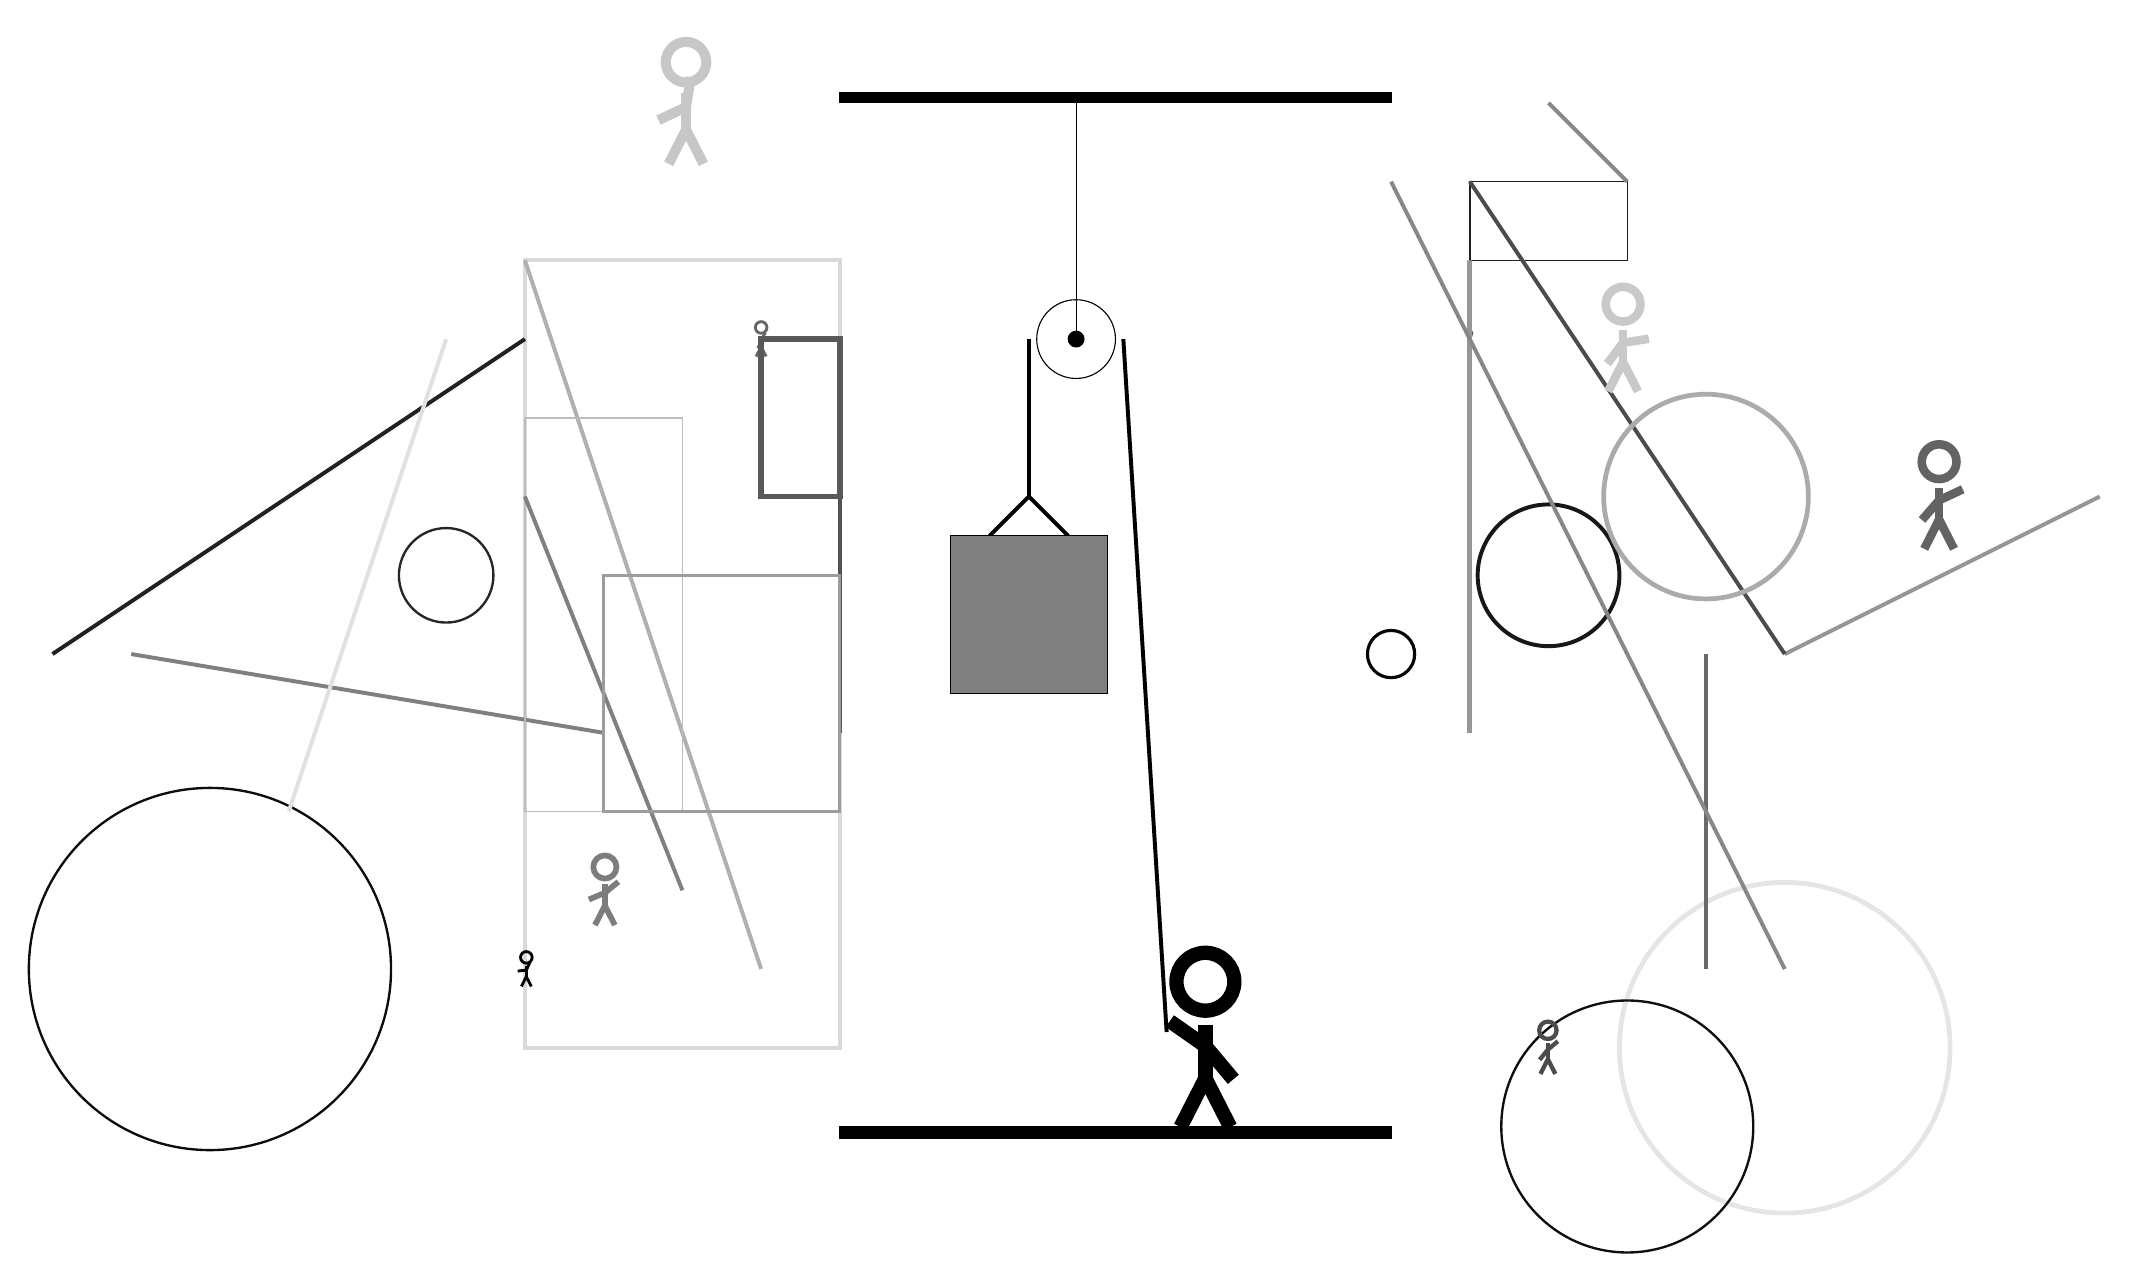
\begin{tikzpicture}
		%%%%% START %%%%%
		
		\draw[fill=black] (-2, 10) rectangle (5, 10.125);
		
		\draw[line width=0.5mm, color=black!15] (-2, 8) rectangle (-6, -2);
		
		\draw[line width=0.5mm, color=black!68] (-2, 6) rectangle (-2, 2);
		\draw [line width=0.4mm, color=black!98](5, 3) circle (0.3);
		\draw [line width=0.6mm, color=black!10](10, -2) circle (2.1);
		\draw[line width=0.5mm, color=black!87](-6, 7) -- (-12, 3);
		\draw[line width=0.5mm, color=black!41](10, 3) -- (14, 5);
		
		\draw [line width=0.3mm, color=black!94](8, -3) circle (1.6);
		
		\node[line width=0.6mm, color=black!70] at (7, -2) {\Strichmaxerl[3][51][40]};
		\draw [line width=0.4mm, color=black!15](5, 8) circle (0.0);
		\draw [line width=0.3mm, color=black!85](-7, 4) circle (0.6);
		
		\node[line width=0.4mm, color=black!51] at (-5, 0) {\Strichmaxerl[4][23][39]};
		\draw [line width=0.3mm, color=black!95](-10, -1) circle (2.3);
		\node[line width=0.2mm, color=black!60] at (-3, 7) {\Strichmaxerl[2][68][62]};
		
		\draw[line width=0.2mm, color=black!88] (6, 9) rectangle (8, 8);
		\draw[line width=0.5mm, color=black!50](-5, 2) -- (-11, 3);
		\draw[line width=0.5mm, color=black!31](-3, -1) -- (-6, 8);
		
		\draw[line width=0.7mm, color=black!65] (-2, 5) rectangle (-3, 7);
		
		\draw [line width=0.5mm, color=black!91](7, 4) circle (0.9);
		\node[line width=0.2mm, color=black!99] at (-6, -1) {\Strichmaxerl[2][5][66]};
		
		\draw[line width=0.5mm, color=black!70](6, 9) -- (10, 3);
		\draw[line width=0.5mm, color=black!59](9, -1) -- (9, 3);
		
		\node[line width=0.4mm, color=black!63] at (6, 7) {\Strichmaxerl[1][89][62]};
		
		\node[line width=0.4mm, color=black!21] at (8, 7) {\Strichmaxerl[6][53][9]};
		\node[line width=0.3mm, color=black!61] at (12, 5) {\Strichmaxerl[6][49][25]};
		\draw[line width=0.6mm, color=black!41] (6, 2) rectangle (6, 8);
		
		\draw[line width=0.5mm, color=black!47](10, -1) -- (5, 9);
		\draw [line width=0.6mm, color=black!33](9, 5) circle (1.3);
		\draw[line width=0.2mm, color=black!26] (-4, 6) rectangle (-6, 1);
		
		\draw[line width=0.5mm, color=black!50](-4, 0) -- (-6, 5);
		\draw[line width=0.5mm, color=black!47](7, 10) -- (8, 9);
		\draw[line width=0.5mm, color=black!12](-7, 7) -- (-9, 1);
		
		\draw[line width=0.4mm, color=black!39] (-2, 1) rectangle (-5, 4);
		\node[line width=0.6mm, color=black!22] at (-4, 10) {\Strichmaxerl[7][25][81]};
		
		\draw (1, 7) circle (0.5);
		\draw[fill=black] (1, 7) circle (0.1);
		\draw (1, 10) -- (1, 7);
		
		\draw[line width=0.5mm] (-0.1, 4.5) -- (0.4, 5.0) -- (0.9, 4.5);
		\draw[fill=black!50] (-0.6, 4.5) rectangle (1.4, 2.5);
		
		\draw[line width=0.5mm] (0.4, 7) -- (0.4, 5.0);
		\centerarc[line width=0.5mm](1, 7)(0:180:0.6);
		\draw[line width=0.5mm](1.6, 7) -- (2.15, -1.8);
		
		\node at (2.6, -1.9) {\Strichmaxerl[10][-35][-50]};
		
		\draw[fill=black] (-2, -3) rectangle (5, -3.15);
		
		%%%%% END %%%%%
	\end{tikzpicture}
\end{document}